\documentclass[../main.tex]{subfiles}

\begin{document}

\chapter{Hierarchical Clustering Model} \label{hierarchical_clustering_model}

\begin{itemize}
    \item What are important variables in the model?
    \item How to visualize results from the model?
    \\~\\
\end{itemize}

In this chapter, we are going to talk about how we use Hierarchical Clustering to classify companies into new sectors. We are going to talk about 2 important variables. The first is the linkage method and the second is the number of new sectors we want. After that, we'll show how we visiualize the new sectors.

\begin{table}[h!]
    \centering
    \begin{tabular}{| c | c |}
        \hline
        &  \\
        RG-1 & Utilize data-driven algorithms to derive a truly objective classification heuristic. \\
        & \\
        \hline
    \end{tabular}
\end{table}

\section{HCA Description}

Hierarchical clustering is an algorithm that groups similar objects into groups called clusters. The endpoint is a set of clusters, where each cluster is distinct from each other cluster, and the objects within each cluster are broadly similar to each other. It builds a tree and we can get whatever number of groups we want depending on how we cut it horizontally. Below is a simple example.

\begin{figure}[H]
    \centering
    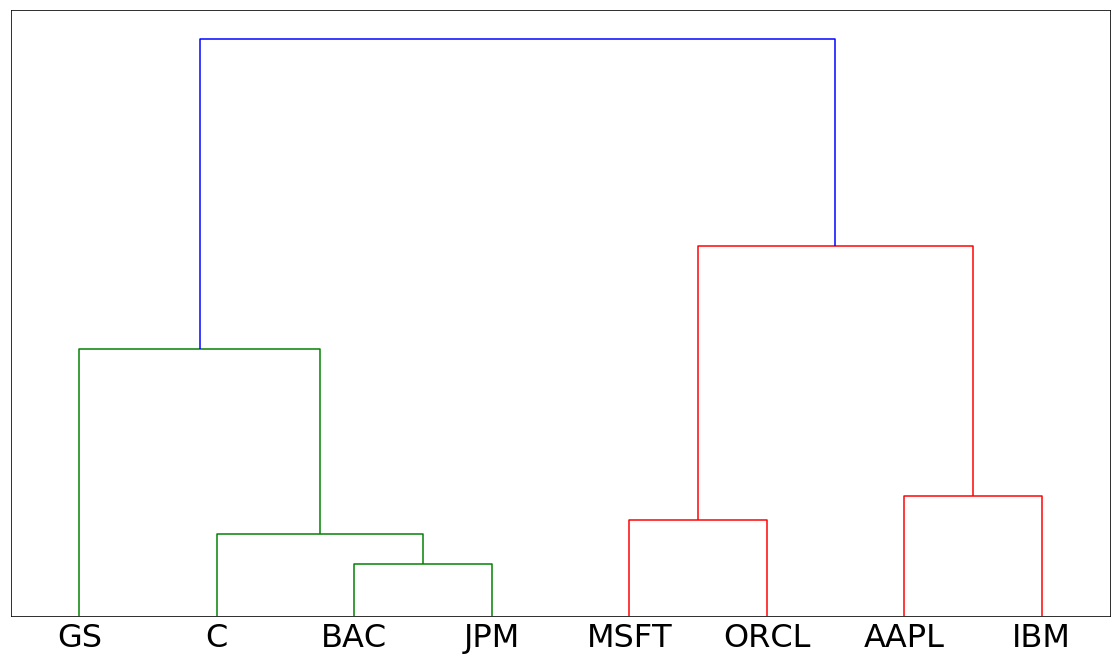
\includegraphics[scale=0.4]{images/tree.png}
    \caption{hierarchical_clustering_model:tree}
    \label{fig:hierarchical_clustering_model:tree}
\end{figure}

\section{Linkage Methods}

The most important thing for this model is how to measure the distance between 2 clusters. There are several ways to calculate it and we call these ways linkage methods. We test 4 common linkage methods in our model. They are called "single", "average", "complete" and "ward". Below are detailed formulas.

For all points \textit{i} in cluster \textit{u} and \textit{j} in cluster \textit{v},
\begin{itemize}
\item Single
$$ d(u,v) = min(d(u[i],v[j])) $$
\item Complete
$$ d(u,v) = max(d(u[i],v[j])) $$
\item Average
$$ d(u,v) = \sum_{ij}{\frac{d(u[i],v[j])}{|u|*|v|}} $$
\item Ward
$$ d(u,v) = \sqrt{\frac{|v|+|s|}{|v|+|u|}d(v,s)^2 + \frac{|v|+|t|}{|v|+|u|}d(v,t)^2 - \frac{|v|}{|v|+|u|}d(s,t)^2} $$
\end{itemize}
where \textit{u} is the newly joined cluster consisting of clusters \textit{s} and \textit{t}, $|*|$ is the cardinality of its argument.

\section{Number of Sectors}

Another important variable is the number of new sectors. How many new sectors should we have? 10? 20? 100? We don't know. Therefore, we test different choices from 5 groups to 19 groups.

\section{Results and Visualization}

After we select the linkage method and the number of new sectors, we use Python scikit-learn package to run hierarchical clustering to get one group of results. To see our results clearly, we use sankey diagram to visualize them. As mentioned above, we have 4 linkage methods and 15 numbers of groups. So we have 60 groups of results in total. Below is the visualization of part of them.

\begin{figure}[h!]
    \centering
    \fbox{
    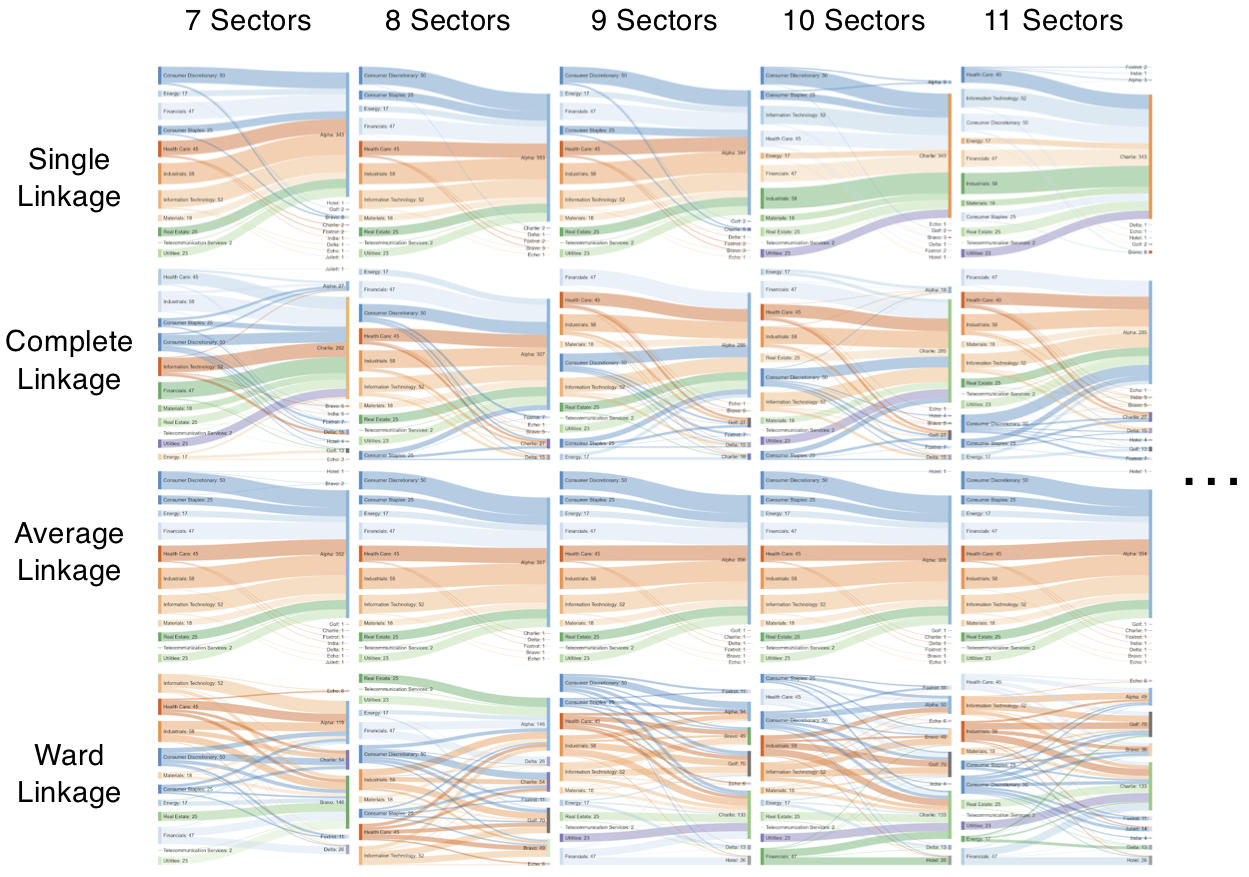
\includegraphics[width=.95\linewidth]{images/search_space_partial.png}
    }
    \caption{Learned sectors partial search space visualization.}
    \label{fig:hierarchical_clustering_model:partial_search_space}
\end{figure}

The question is which group is the best? And more importantly, is it better than the traditional sectors? From next chapter, we are going to answer these questions.

\end{document}